\documentclass{article}

\usepackage{graphicx} % Required for inserting images
\usepackage{CJKutf8}
\usepackage{graphicx}

\title{2023校内赛}
\author{hongyh494}
\date{August 2023}

\begin{document}
\begin{CJK}{UTF8}{gbsn}
\maketitle

\section{模型建立}
GUIDE决策树分类算法:我们使用GUIDE决策树分类算法进行分类预测。GUIDE算法可容纳的自变量维度极高,且可对不同变量进行数值型(numeric),类别型(category),循环型(cyclic)的分类,极大地保留了变量本身的类型属性,再将自变量x与因变量Y之间的相关程度,通过Chi-squared检验来进行相关性排名和p-value计算,得到变量的排名列表与置信度,再通过变量排名列表选择分类结点对样本数据进行决策分类。
\section{模型求解}
    \subsection{A2年龄与生活、饮食习惯}
        \subsubsection{数据预处理}
我们将年龄进行分层处理,依据7-12岁为少儿;13-17岁为青少年;18-45岁为青年;46-69岁为中年;69岁以上为老年。样本中年龄最大值为123,年龄最小值为29,其中>=100岁的样本仅有4例。因此我们决定剔除>=100岁的样本减小误差,并分类成18-45岁为1类,46-69岁为2类,69岁以上为3类,共三类人群用GUIDE决策树算法,将生活、饮食习惯设置为变量得到分类结果。
首先我们得到GUIDE决策树算法中对变量与因变量年龄之间相关性的评分,一下是分类置信度\>99\%的前20名变量,与决策树可视化。
\\
模型求解:
\begin{figure}[htbp]
    \flushleft
    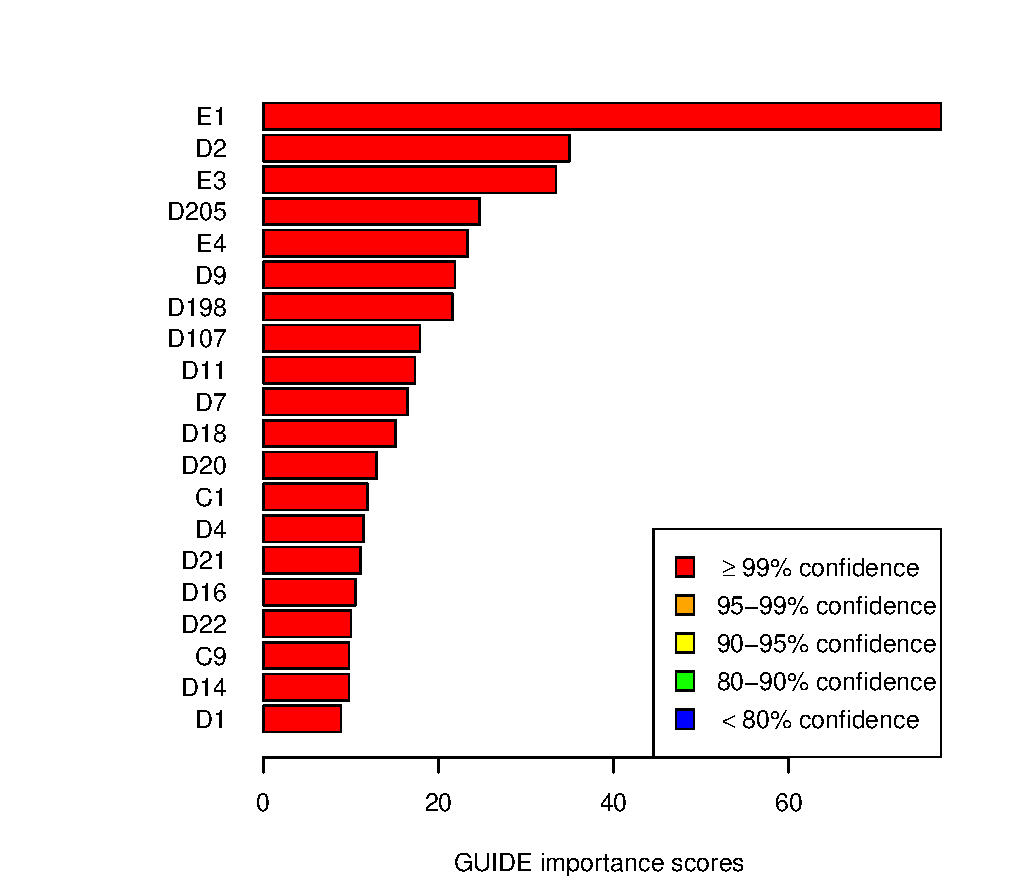
\includegraphics[scale=0.6]{A2_imp.eps}
    \caption{年龄与生活、饮食习惯的决策树可视化}
    \label{}
\end{figure}
\begin{figure}[htbp]
    \flushleft
    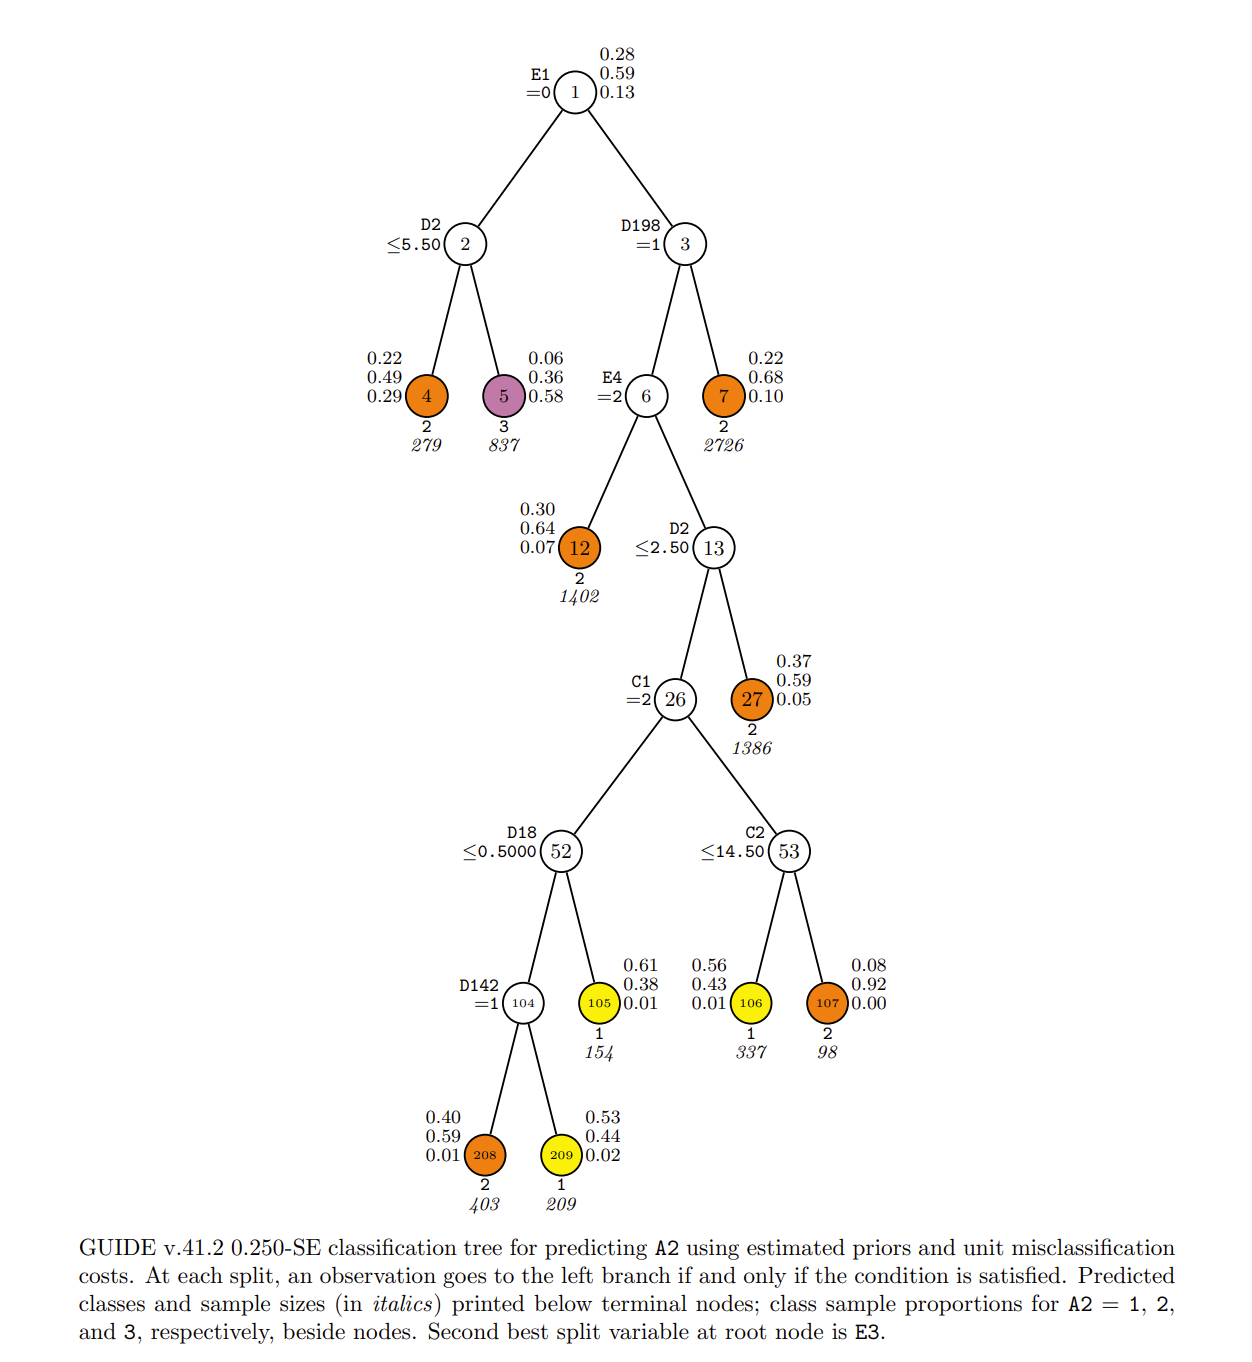
\includegraphics[scale=0.6]{A2_tree.png}
    \caption{年龄与生活、饮食习惯的决策树可视化}
    \label{}
\end{figure}
可以看到E1,D2,E3,D205,E4因素对分类结果影响较大,也即不同年龄的人在工作属于的活动,一周在家吃早餐的次数,是否参加体育锻炼,是否吃其它饮料,是否参加体育锻炼在这些方面差异较大。通过决策树模型我们也可以发现:18~45岁的青年人群主要从事中重度的工作,喝果汁,体育锻炼强度大,一周在家吃早餐的天数少(<=2),其中不饮酒的人更愿意在单位食堂吃晚餐且不爱吃干豆;46~69的中年人群体分支较多:中年人中的离退休人群较老年人不爱在家中吃早饭;仍在工作的中年人较不爱喝果汁,体育锻炼强度小,较青年人爱在家吃早饭,也更爱吃干豆。老年人群体一周在家吃早餐的时间在6天以上。\\

\subsection{A3性别与生活、饮食习惯}
我们得到GUIDE决策树算法中对变量与因变量性别之间相关性的评分,一下是分类置信度>99\%的前20名变量,与决策树可视化。
\begin{figure}[htbp]
    \flushleft
    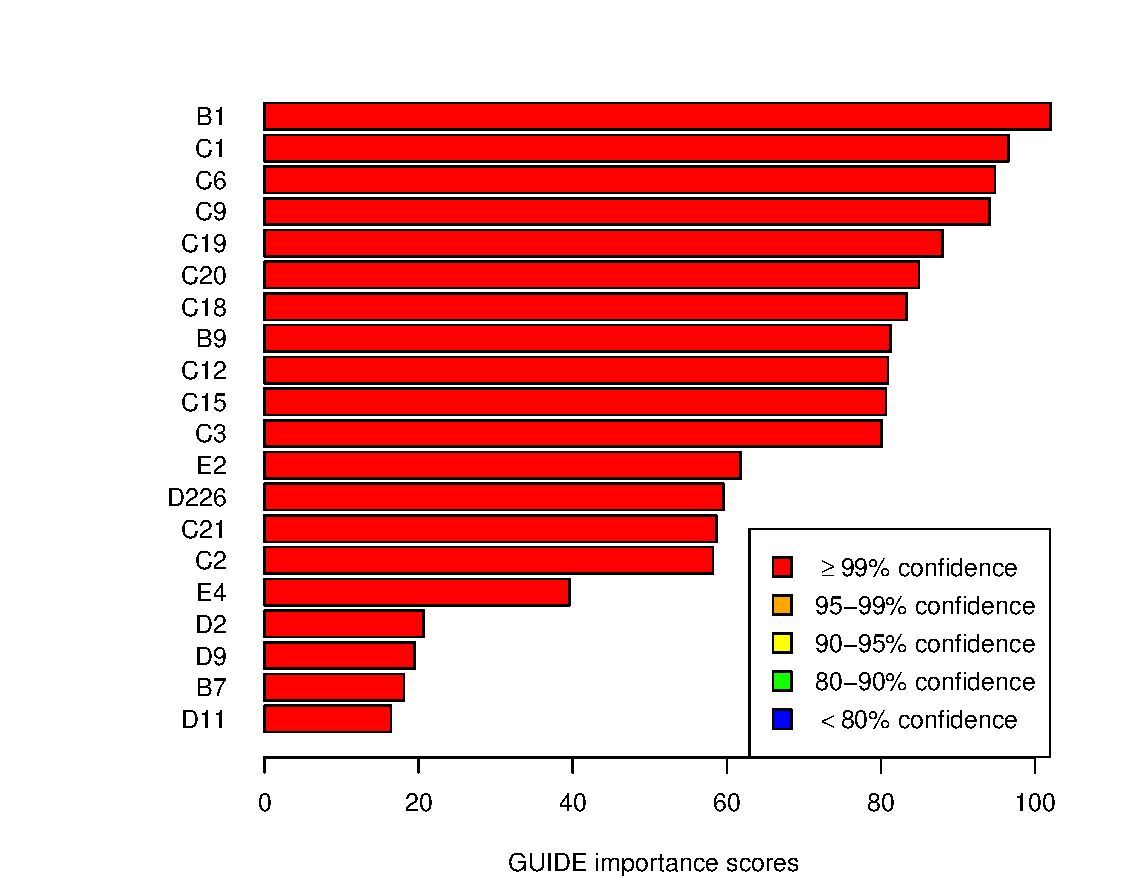
\includegraphics[scale=0.6]{A3_imp.eps}
    \caption{性别vs生活、饮食习惯变量的重要性排名}
    \label{}
\end{figure}
\begin{figure}[htbp]
    \flushleft
    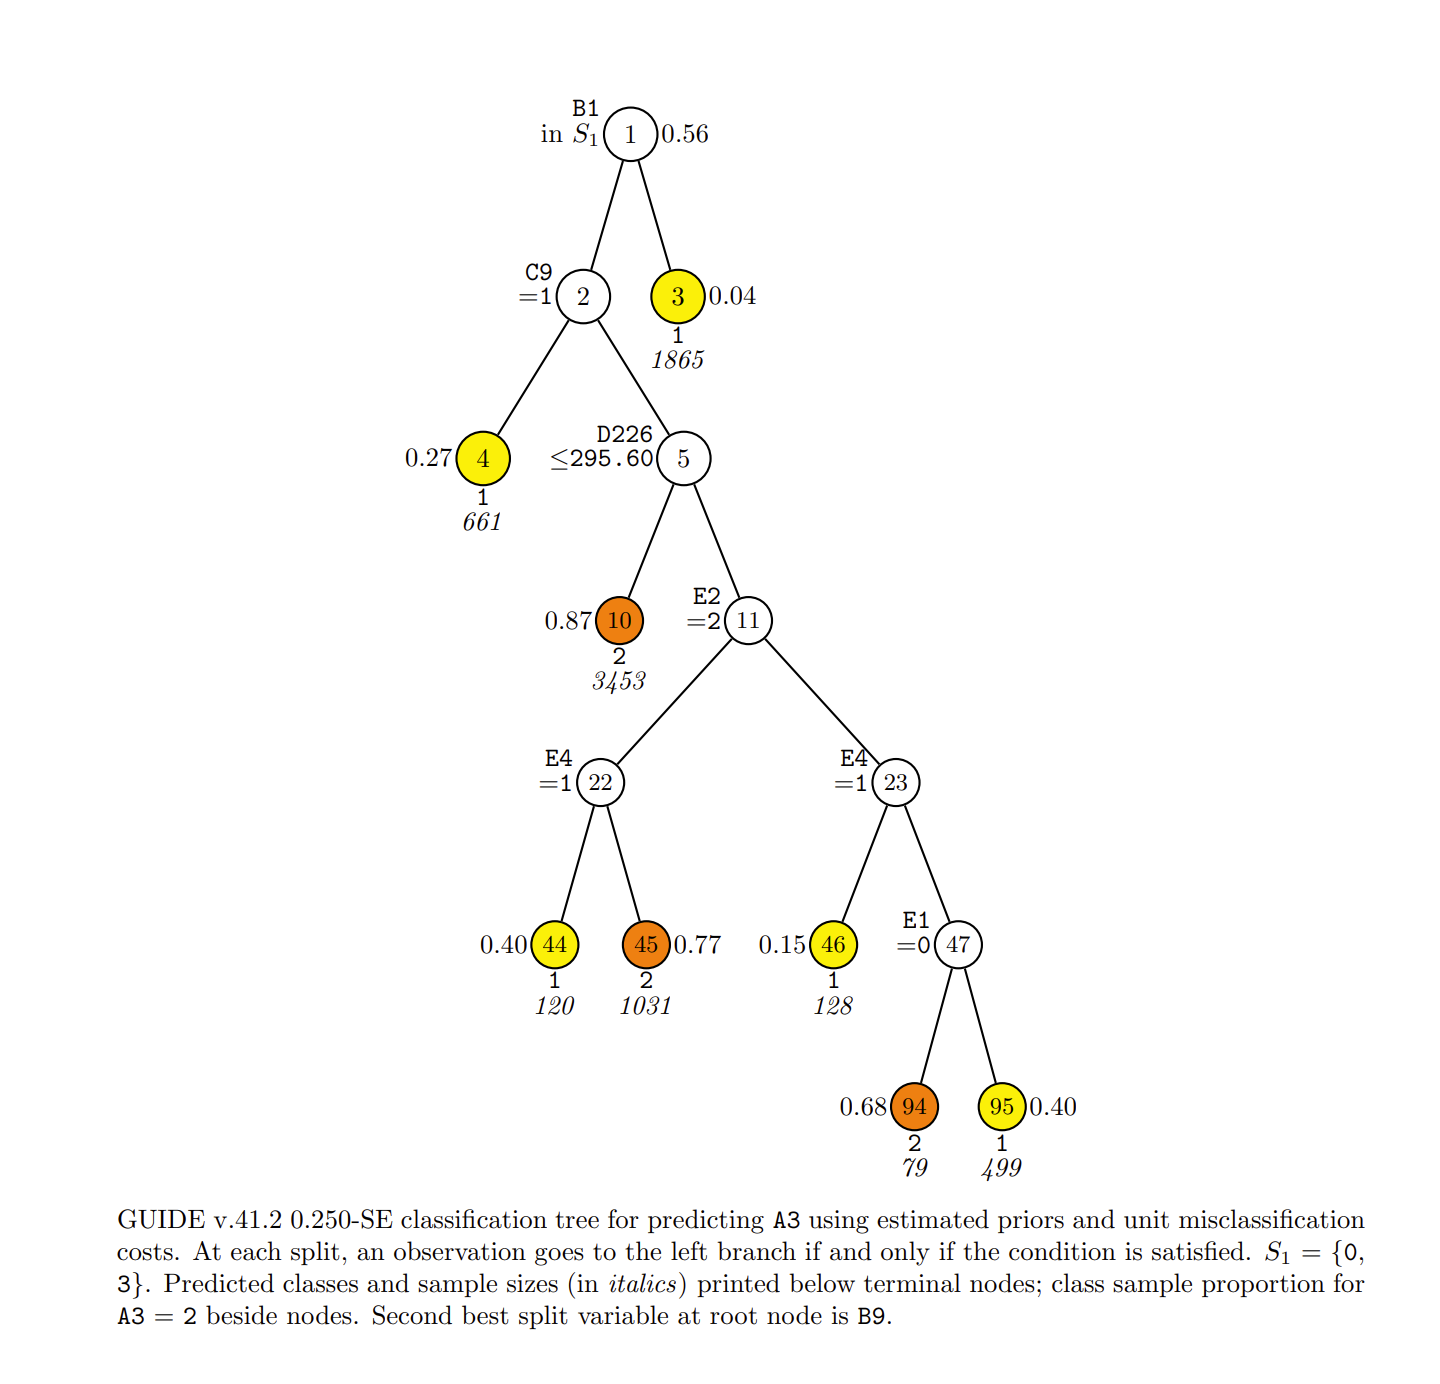
\includegraphics[scale=0.6]{A3_tree.png}
    \caption{性别与生活、饮食习惯的决策树可视化}
    \label{}
\end{figure}

\subsection{A6文化程度与生活、饮食习惯}
我们得到GUIDE决策树算法中对变量与因变量文化程度之间相关性的评分,一下是分类置信度>99\%的前20名变量,与决策树可视化。
\begin{figure}[htbp]
    \flushleft
    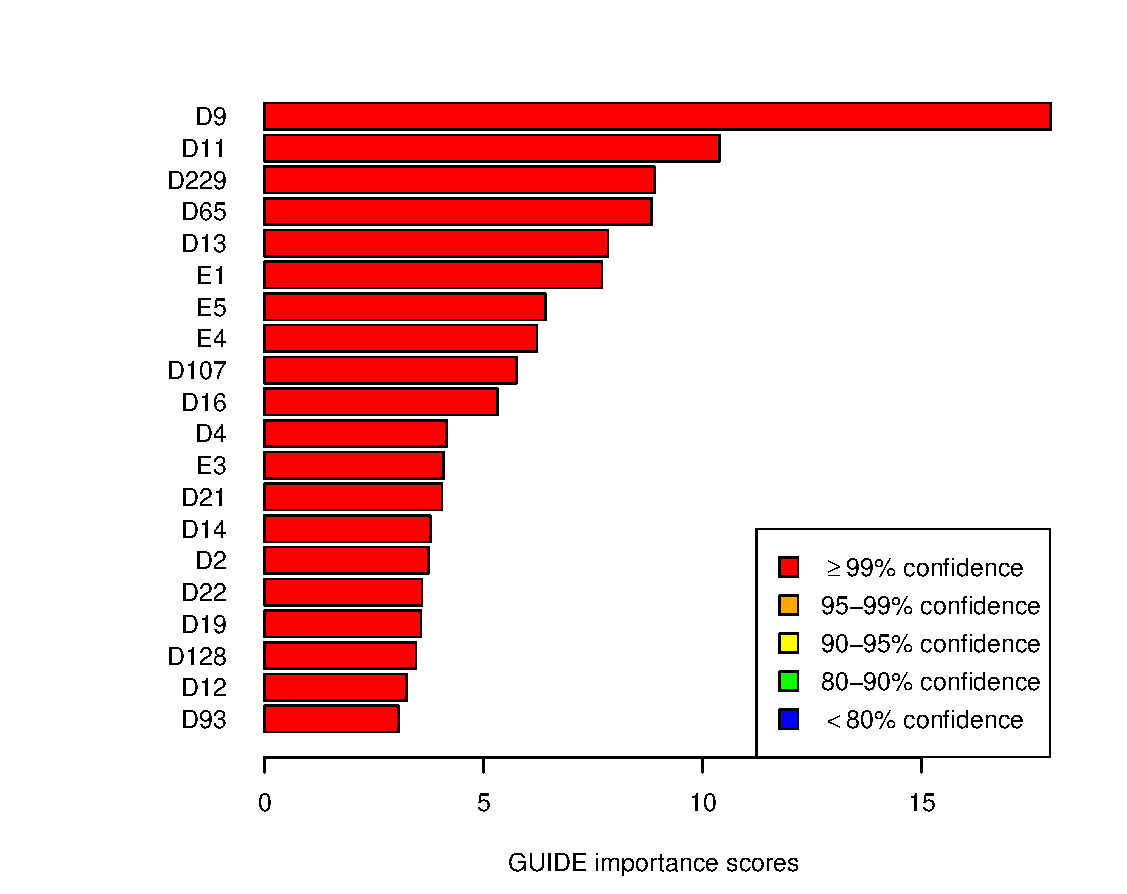
\includegraphics[scale=0.5]{A6_imp.eps}
    \caption{文化程度vs生活、饮食习惯变量的重要性排名}
    \label{}
\end{figure}
\begin{figure}[htbp]
    \flushleft
    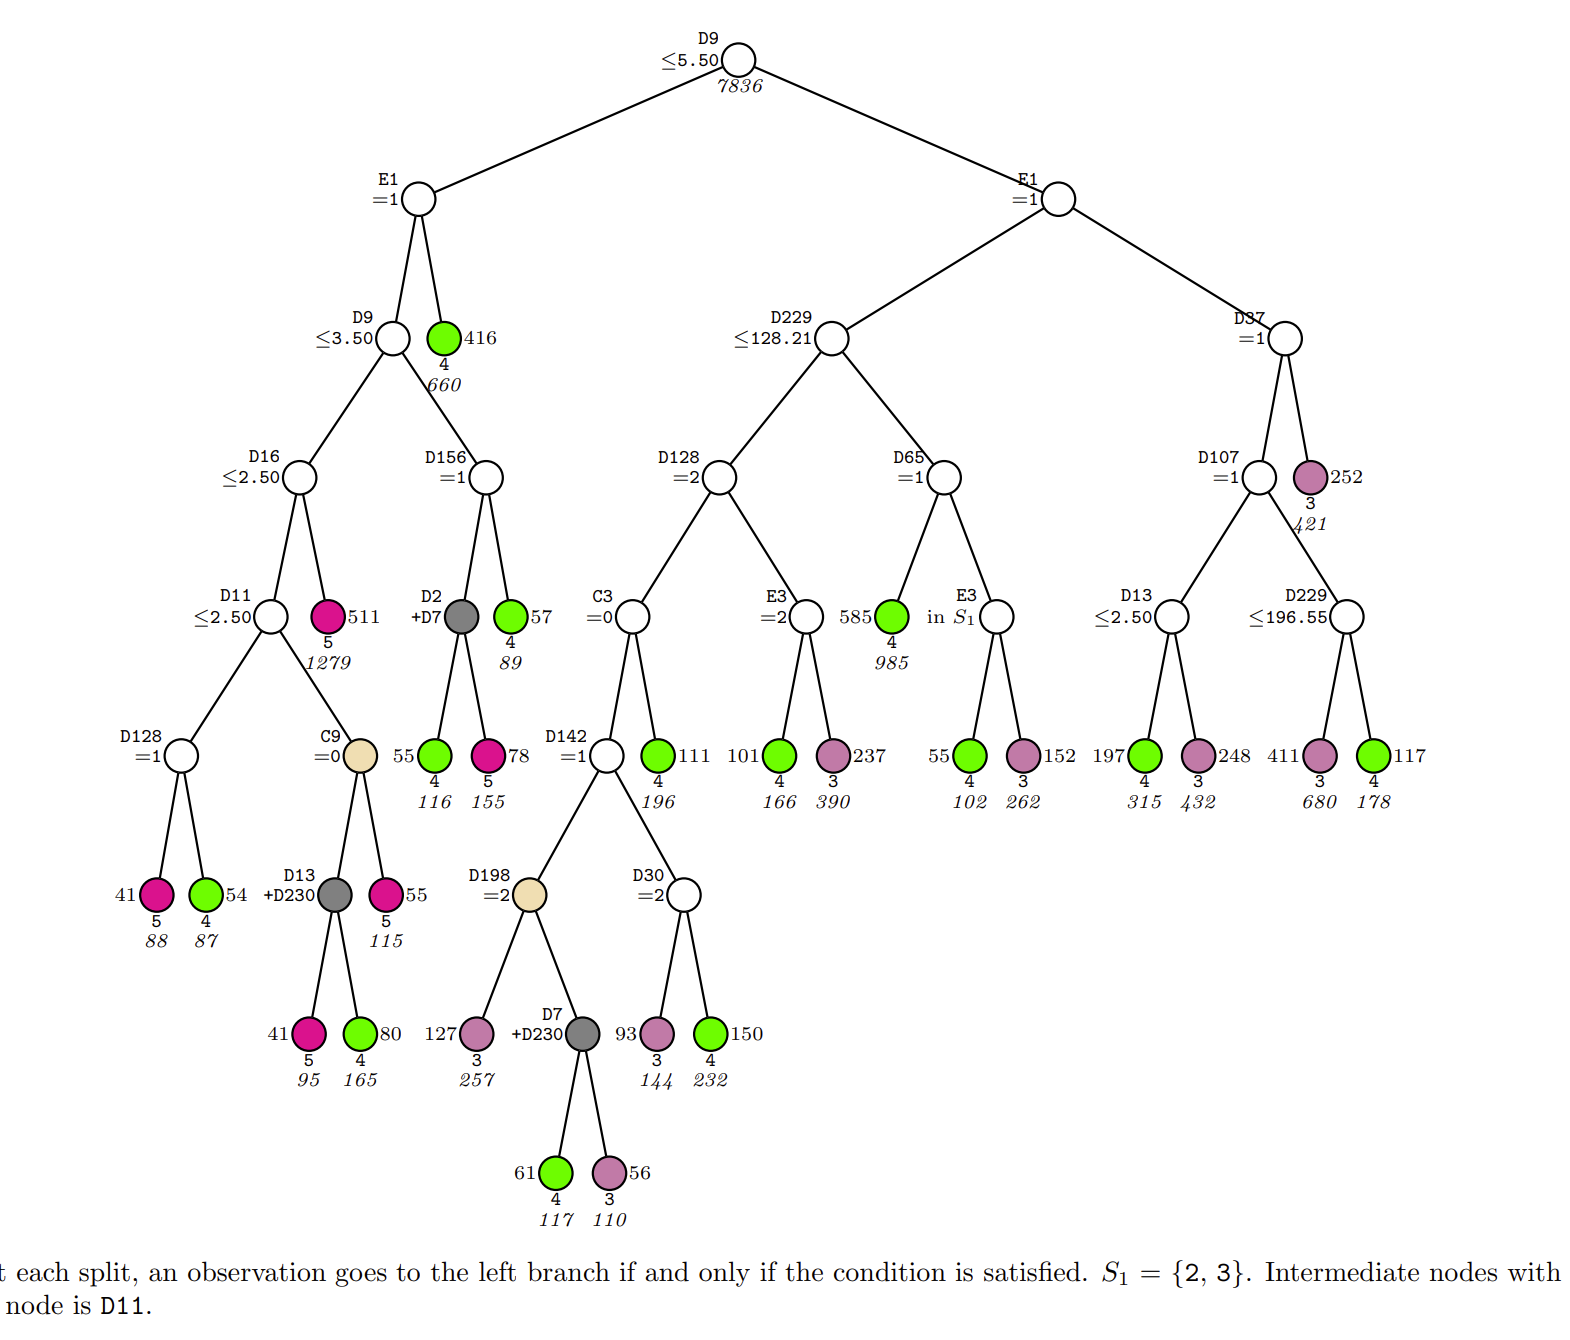
\includegraphics[scale=0.7]{A6_tree.png}
    \caption{文化程度与生活、饮食习惯的决策树可视化}
    \label{}
\end{figure}

\subsection{A7婚姻状况与生活、饮食习惯}
我们得到GUIDE决策树算法中对变量与因变量婚姻状况之间相关性的评分,一下是分类置信度>99\%的前20名变量,与决策树可视化。
\begin{figure}[htbp]
    \flushleft
    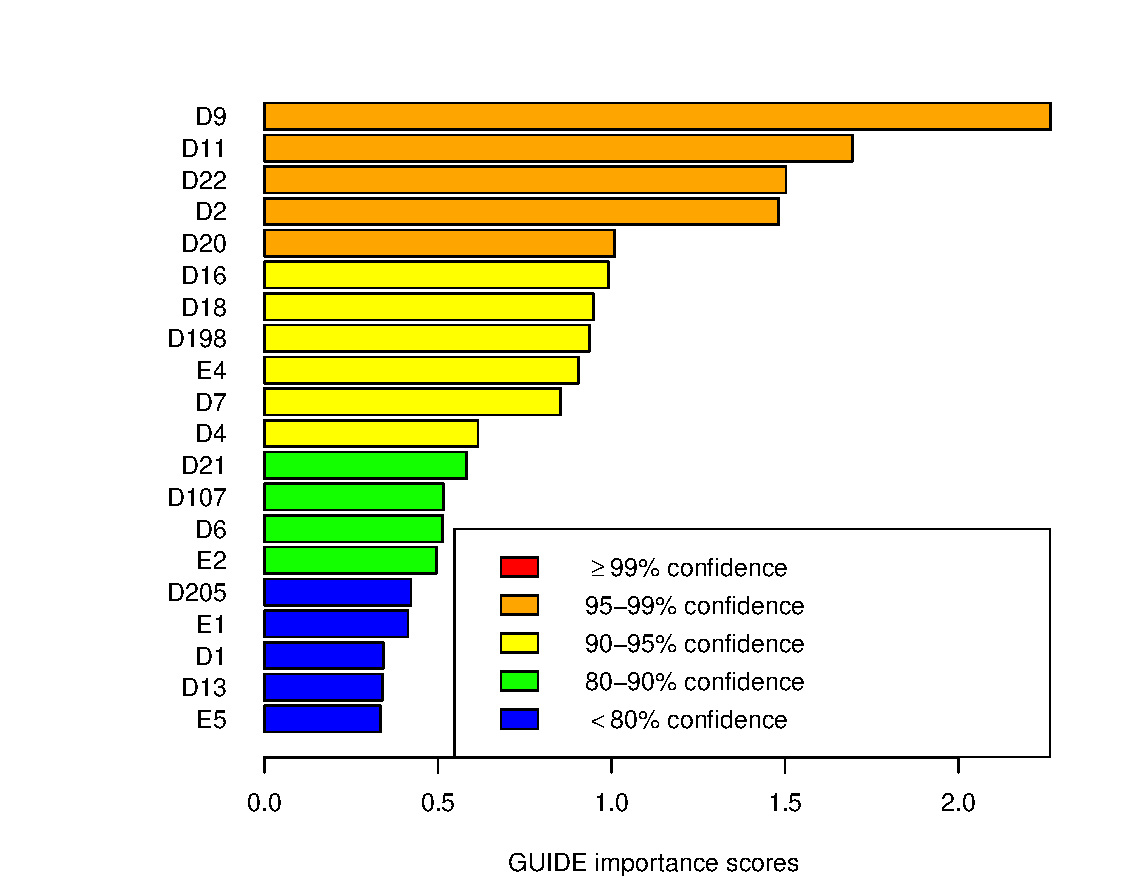
\includegraphics[scale=0.7]{A7_imp.eps}
    \caption{婚姻状况vs生活、饮食习惯的重要性排名}
    \label{}
\end{figure}
\begin{figure}[htbp]
    \flushleft
    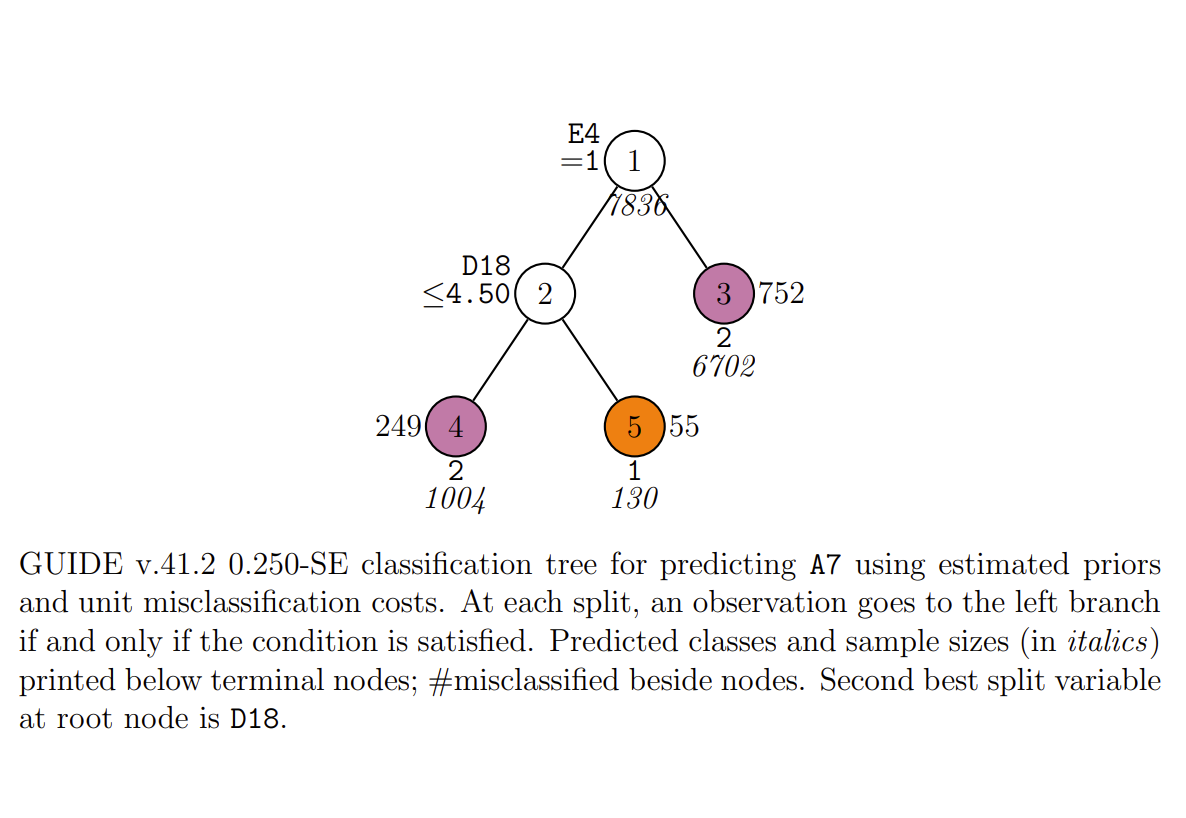
\includegraphics[scale=0.8]{A7_tree.png}
    \caption{婚姻状况与生活、饮食习惯的决策树可视化}
    \label{}
\end{figure}
可以看到未婚人群中参与高强度的体育体育锻炼的人明显更多,且更倾向于在单位食堂吃晚餐;已婚人群更倾向于在家中吃晚餐,且更倾向于做中低强度的运动。

\subsection{A8职业与生活、饮食习惯}
我们得到GUIDE决策树算法中对变量与因变量职业之间相关性的评分,一下是分类置信度>99\%的前20名变量,与决策树可视化。
\begin{figure}[htbp]
    \flushleft
    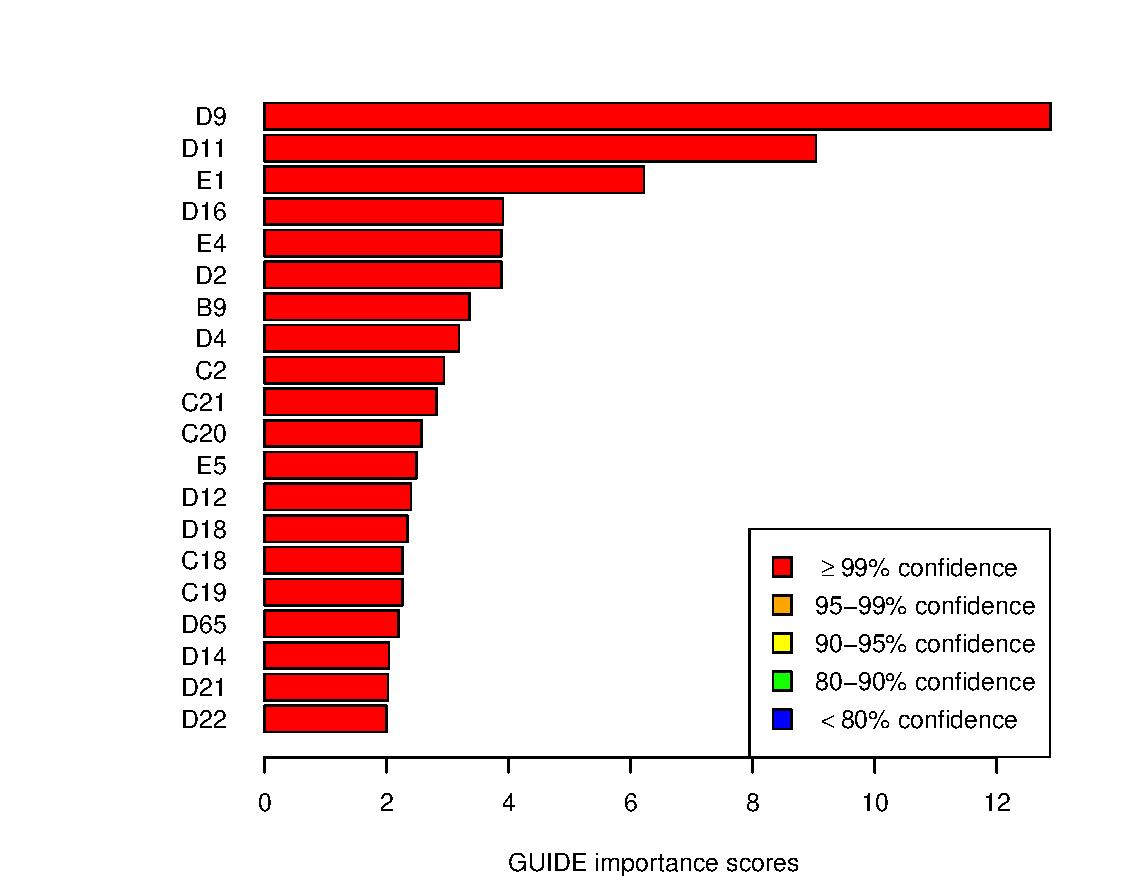
\includegraphics[scale=0.7]{A8_imp.eps}
    \caption{职业vs生活、饮食习惯变量的重要性排名}
    \label{}
\end{figure}
\begin{figure}[htbp]
    \flushleft
    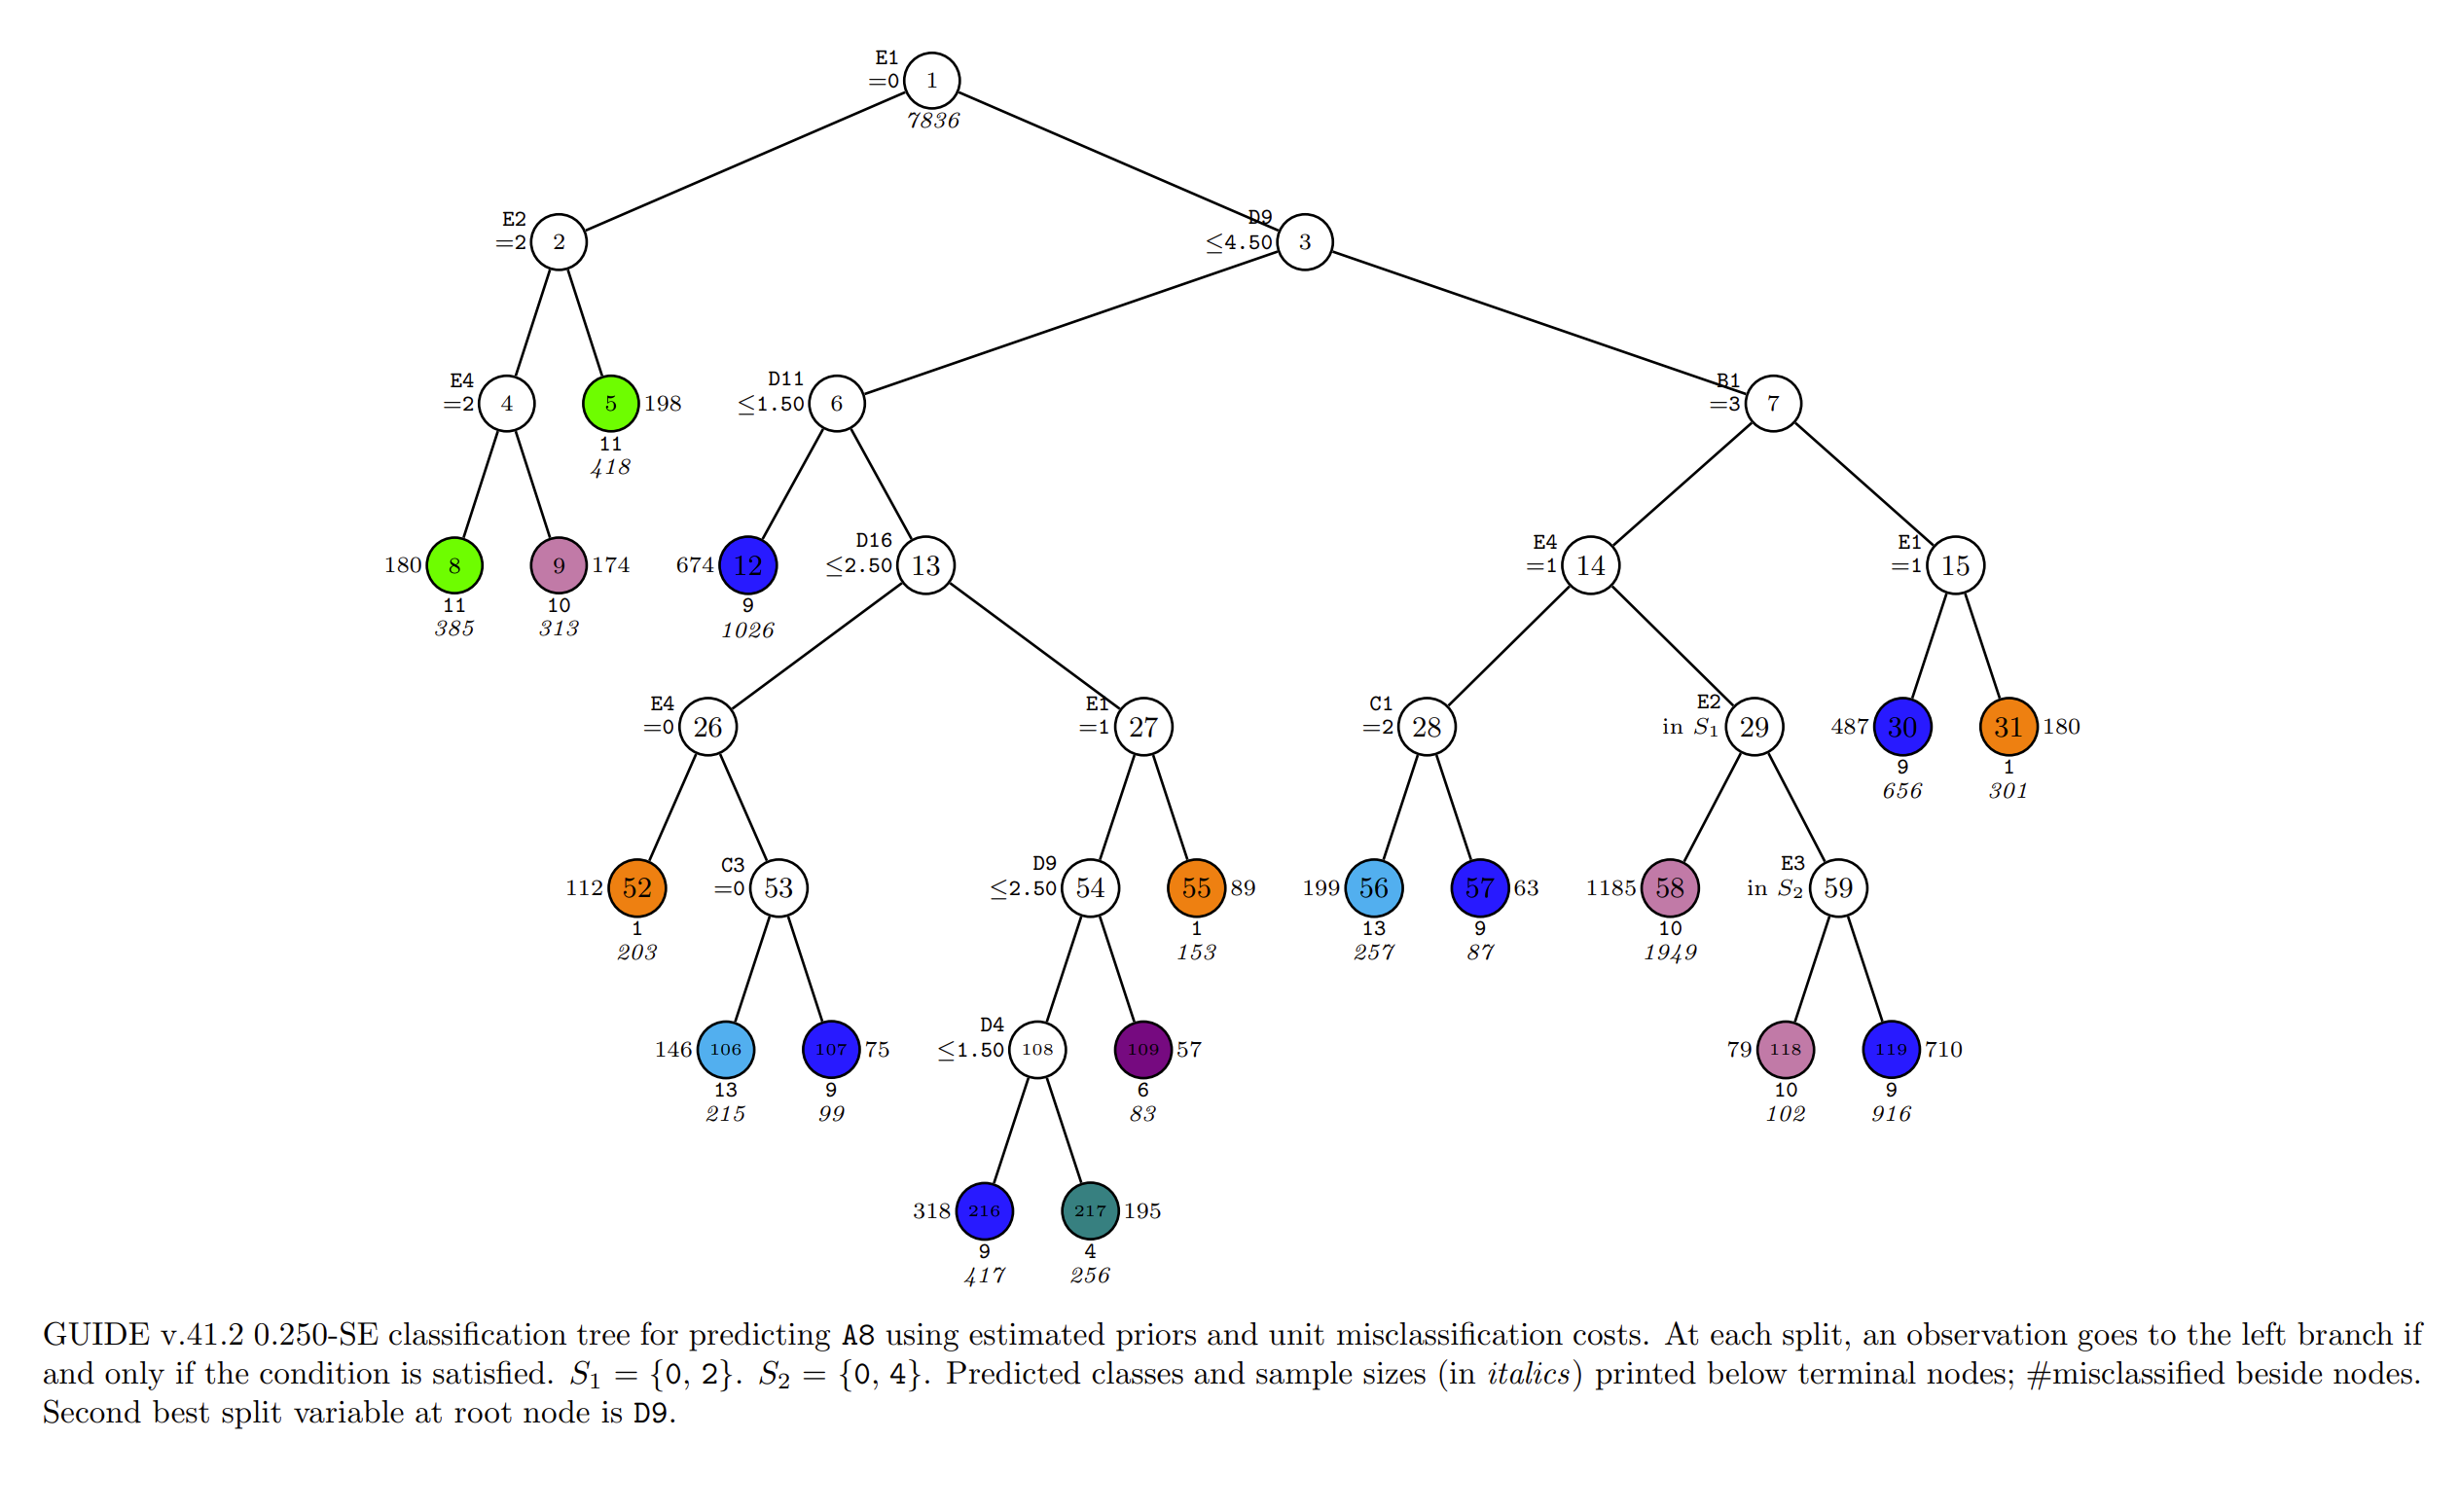
\includegraphics[scale=0.45]{A8_tree.png}
    \caption{职业与生活、饮食习惯的决策树可视化}
    \label{}
\end{figure}

GUIDE
先用随机森林找到最有关联性的变量\\
A3性别:D226,E2休闲、家务活动的强度,B1,C19,B9\\
A6文化程度:D9,E1工作主要属于以下何种活动,D229,D65,D221\\
A7婚姻状况;D18,D22,D16,E1工作主要属于以下何种活动,D14,D13,D229\\
A8职业:E1工作主要属于以下何种活动,D11,B1,E3,D9\\

\section{模型评价与改进}
优点:GUIDE决策树算法可解释性强,可视化能力强,分类处理一目了然。通过对不同的自变量进行数值型与类别型的分类,极大地保留了变量本身离散与连续的属性。且模型训练准确性高,具有很好的应用价值。
缺点:1、决策树算法对变量之间可能存在的相关性无法阐明,可能会造成与因变量联系较强的相关类型的变量只有一种脱颖而出,因此某些人群的较不明显的属性无法一并体现。2、自变量维度过高,决策树算法分类容易省略较多自变量与因变量的相关信息。
模型改进:对多种自变量之间通过算法进行相关性分析,优化相似类型自变量,降维自变量模型。
\end{CJK}
\end{document}
